\documentclass[11pt,a4paper]{article}
			\usepackage[french]{babel}
					
				\usepackage{pifont}  
				\usepackage[utf8x]{inputenc}
				\usepackage[T1]{fontenc} 
				\usepackage{lmodern}			
				\usepackage{fancyhdr}
				\usepackage{textcomp}
				\usepackage{makeidx}
				\usepackage{tabularx}
				\usepackage{multicol}
				\usepackage{multirow}
				\usepackage{longtable}
				\usepackage{color}
				\usepackage{soul}
				\usepackage{boxedminipage}
				\usepackage{shadow}
				\usepackage{framed}			
				\usepackage{array}
				\usepackage{url}
				\usepackage{ragged2e}
				\usepackage{fancybox}
				\newcommand{\cadretitre}[2]{
				  \vspace*{0.8\baselineskip}
				  \begin{center}%
				  \boxput*(0,1){%
					%\colorbox{white}{\Large\textbf{\ #1\ }}%
				  }%
				  {%
					\setlength{\fboxsep}{10pt}%
				    \Ovalbox{\begin{minipage}{.8\linewidth}\begin{center}\Large\sffamily{#2}\end{center}\end{minipage}}}%
				  \end{center}
				  \vspace*{2\baselineskip}
				  }
			
			\makeatletter
			\def\@seccntformat#1{\protect\makebox[0pt][r]{\csname the#1\endcsname\quad}}
			\makeatother

				% Permet d'afficher qqchose à une positin absolue
				\usepackage[absolute]{textpos}
				\setlength{\TPHorizModule}{1cm}
				\setlength{\TPVertModule}{\TPHorizModule}
	
				\usepackage[titles]{tocloft}
				\setlength{\cftbeforesecskip}{0.5ex}
				\setlength{\cftbeforesubsecskip}{0.2ex}
				\addto\captionsfrench{\renewcommand\contentsname{}}
				
				\usepackage[font=scriptsize]{caption}
				
				\usepackage{listings}
\lstdefinestyle{lstverb}
  {
    basicstyle=\footnotesize,
    frameround=tttt, frame=trbl, framerule=0pt, rulecolor=\color{gray},
    lineskip=-1pt,   % pour rapprocher les lignes
    flexiblecolumns, escapechar=\\,
    tabsize=4, extendedchars=true
  }
\lstnewenvironment{Java}[1][]{\lstset{style=lstverb,language=java,#1}}{}
				\ifx\pdfoutput\undefined
					\usepackage{graphicx}
				\else
					\usepackage[pdftex]{graphicx}
				\fi
				\usepackage[a4paper, hyperfigures=true, colorlinks, linkcolor=black, citecolor=blue,urlcolor=blue, pagebackref=true, bookmarks=true, bookmarksopen=true,bookmarksnumbered=true,
                pdfauthor={}, pdftitle={TD Chaines}, pdfkeywords={TD Chaines, },pdfpagemode=UseOutlines,pdfpagetransition=Dissolve,nesting=true,
				backref, pdffitwindow=true, bookmarksnumbered=true]{hyperref}
				\usepackage{supertabular}
				\usepackage[table]{xcolor}
				\usepackage{url}
				\usepackage{caption} 
				\setlength{\parskip}{1.3ex plus 0.2ex minus 0.2ex}
				\setlength{\parindent}{0pt}
				
				\makeatletter
				\def\url@leostyle{ \@ifundefined{selectfont}{\def\UrlFont{\sf}}{\def\UrlFont{\footnotesize\ttfamily}}}
				\makeatother
				\urlstyle{leo}
				
				\definecolor{examplecolor}{rgb}{0.156,0.333,0.443}
				\definecolor{definitioncolor}{rgb}{0.709,0.784,0.454}
				\definecolor{exercisecolor}{rgb}{0.49,0.639,0}
				\definecolor{hintcolor}{rgb}{0.941,0.674,0.196}
				\definecolor{tableHeadercolor}{rgb}{0.709,0.784,0.454}
				\definecolor{tablerowAltcolor}{rgb}{.866,.905,.737}
				\definecolor{tablerowAlt2color}{rgb}{.968,.976,.933}
				\definecolor{verylightgray}{rgb}{0.98,0.98,0.98}
				
				\newenvironment{fshaded}{
				\def\FrameCommand{\fcolorbox{framecolor}{shadecolor}}
				\MakeFramed {\FrameRestore}}
				{\endMakeFramed}
				
				\newenvironment{fexample}[1][]{\definecolor{shadecolor}{rgb}{.913,.913,.913}
				\definecolor{framecolor}{rgb}{.156,.333,.443}
				\begin{fshaded}}{\end{fshaded}} 
				
				\newenvironment{fdefinition}{\definecolor{shadecolor}{rgb}{.913,.913,.913}
				\definecolor{framecolor}{rgb}{.709,.784,.454}
				\begin{fshaded}}{\end{fshaded}}
				
				\newenvironment{fexercise}{\definecolor{shadecolor}{rgb}{.913,.913,.913}
				\definecolor{framecolor}{rgb}{.49,.639,0}
				\begin{fshaded}}{\end{fshaded}}
				
				\newenvironment{fhint}{\definecolor{shadecolor}{rgb}{.913,.913,.913}
				\definecolor{framecolor}{rgb}{.941,.674,.196}
				\begin{fshaded}}{\end{fshaded}}	
				
				\newcommand{\PreserveBackslash}[1]{
				\let\temp=\\#1\let\\=\temp
				}
				\let\PBS=\PreserveBackslash
				\newcolumntype{A}{>{\PBS\raggedright\small\hspace{0pt}}X}
				\newcolumntype{L}[1]{>{\PBS\raggedright\small\hspace{0pt}}p{#1}}
				\newcolumntype{R}[1]{>{\PBS\raggedleft\small\hspace{0pt}}p{#1}}
				\newcolumntype{C}[1]{>{\PBS\centering\small\hspace{0pt}}p{#1}}
				
				\makeindex
				
				\title{TD Chaines}	
			\date{}
			\author{\scriptsize{}}
			\definecolor{light-gray}{gray}{0.8}
			\renewcommand{\headrulewidth}{0pt}
			\fancyhead[L]{
				\footnotesize\textsc{Haute \'Ecole de Bruxelles}\\
	    			\footnotesize\textsc{\'Ecole Sup\'erieure d'Informatique}
			}
			\fancyhead[R]{
				\footnotesize{Bachelor en Informatique}\\
				\footnotesize{Laboratoires Java} - 
			\footnotesize{1\`ere ann\'ee}}
				\fancyfoot[L]{ }
				\fancyfoot[C]{}
				\fancyfoot[R]{\scriptsize{\textcolor{gray}{version 2014-2015 (\today)}}}
				\pagestyle{plain}
				\reversemarginpar
				\usepackage{rotating}						
				\begin{document}
					\begin{textblock}{9}(2,3.2)
						
\includegraphics[width=2cm]{../../../_templates/java/icons/logo-esi}
					\end{textblock}
				
				
				
				
				%\maketitle
				\cadretitre{TD1}{TD Chaines}
				\thispagestyle{fancy}
        \marginpar{\begin{sideways}
            \begin{minipage}[t]{1cm}
            \begin{tiny}
            
\includegraphics[width=1\linewidth,height=1\textheight,keepaspectratio=true]{../../../_templates/java/icons/cc-gris.jpg}
			\end{tiny}
			\end{minipage}
            \begin{minipage}[b]{19cm}
            \begin{tiny}
            \textcolor{gray}{Distribué sous licence Creative Commons Paternité - Partage à l'Identique 2.0 Belgique 
            (\texttt{http://creativecommons.org/licenses/by-sa/2.0/be/})
			\vspace{-1em}
			\\Les autorisations au-delà du champ de cette licence peuvent être obtenues à 
			\texttt{http://www.heb.be/esi}
			- \texttt{mcodutti@heb.be}
			}\end{tiny}
			\end{minipage}
        \end{sideways}}
            \begin{abstract}
			Voyons ici les caract\`eres et les chaines de caract\`eres.
    
            \par
        \end{abstract}
				\vspace{-2em}\tableofcontents
				\pagestyle{plain}
            \clearpage
            \fancyhead[L,C,R]{}
            \fancyfoot[L,C]{}
            \fancyfoot[R]{ \scriptsize{\textcolor{gray}{
				TDChaine - page \thepage}}}
				\thispagestyle{fancy}
				\pagestyle{fancy}
	   
            \section{Les chaines}
        Nous avons d\'efini deux types de variables qui permettent de stocker du texte :
        
					\begin{itemize}
				
			\item 
            le caract\`ere (pour les diff\'erentes lettres et symboles qui apparaissent sur le clavier de votre
            ordinateur, par exemple 'a', 'B', ' ?', '3', '@', etc.) 
          
			\item et la chaine (qui est un assemblage de plusieurs caract\`eres)
					\end{itemize}
				
            \par
        
        Observez la petite nuance d'\'ecriture : 
        un caract\`ere sera entour\'e d'apostrophes (ou simples guillemets) (\verb@’ ’@) 
        et une chaine de doubles guillemets (\verb@" "@).
      
            \par
        
        La \textbf{taille (ou longueur) d'une chaine} est le nombre de caract\`eres qu'elle contient. 
        Remarquez qu'une chaine peut \^etre vide, mais pas un caract\`ere ! Ne confondez pas la chaine vide ("", de
        taille nulle) avec le caract\`ere blanc (' ') qui contient l'espace s\'eparant 2 mots d'un texte et
        que vous obtenez en enfon\c cant la touche d'espacement au bas du clavier.
		
            \par
        \subsection{Manipuler les caract\`eres}
        Introduisons quelques fonctions (ou primitives) agissant sur les caract\`eres. Leur \'ecriture
        s'apparente \`a celle de modules que vous pourrez utiliser tels quels dans les exercices. 
      
            \par
        \begin{verbatim}
        estLettre(car : caractère) → booléen
      \end{verbatim}
        Cette fonction indique si un caract\`ere est une lettre. Par exemple elle retourne vrai pour 'a',
        'e', 'G', 'K', mais faux pour '4', '\$', '@'. . .
      
            \par
        
        Si on veut savoir si une lettre est une minuscule ou majuscule, on utilisera les fonctions
        analogues
      
            \par
        \begin{verbatim}
        estMinuscule(car : caractère) → booléen
      \end{verbatim}
        et
      
            \par
        \begin{verbatim}
        estMajuscule(car : caractère) → booléen
      \end{verbatim}
        Il va de soi que si \verb@car@ n'est pas une lettre, ces deux fonctions retournent faux.
      
            \par
        \begin{verbatim}
        estChiffre(car : caractère) → booléen
      \end{verbatim}
        Cette fonction permet de savoir si un caract\`ere est un chiffre. Elle retourne vrai uniquement
        pour les dix caract\`eres '0', '1', '2', '3', '4', '5', '6', '7', '8' et '9' et faux dans tous les autres
        cas.
      
            \par
        
        On peut aussi convertir une majuscule en minuscule, gr\^ace \`a la fonction :
      
            \par
        \begin{verbatim}
        majuscule(car : caractère) → caractère
      \end{verbatim}
        Par exemple, si \verb@car@ vaut \verb@’h’@, 
        cette fonction retourne \verb@’H’@. L'op\'eration inverse se fait avec :
      
            \par
        \begin{verbatim}
        minuscule(car : caractère) → caractère
      \end{verbatim}
        Il peut aussi \^etre pratique de connaitre la position d'une lettre dans l'alphabet. Ceci se fera
        \`a l'aide de la fonction :
      
            \par
        \begin{verbatim}
        numLettre(car : caractère) → entier
      \end{verbatim}
        qui retourne toujours un entier entre 1 et 26. Par exemple numLettre('E') donnera 5, ainsi
        que numLettre('e'), cette fonction traite donc de la m\^eme mani\`ere les majuscules et les
        minuscules. En vertu de ce qui a \'et\'e \'ecrit plus haut, numLettre retournera aussi 5 pour les
        caract\`eres '\'e', '\`e', '\^e', '\"e'. . .). N.B. : attention, il est interdit d'utiliser cette fonction si le
        caract\`ere n'est pas une lettre !
      
            \par
        
        Il peut \^etre utile d'avoir un outil qui fait l'op\'eration inverse, \`a savoir associer la lettre de
        l'alphabet correspondant \`a une position donn\'ee. Pour cela, nous aurons :
      
            \par
        \begin{verbatim}
        lettreMaj(n : entier) → caractère
      \end{verbatim}
        et
      
            \par
        \begin{verbatim}
        lettreMin(n : entier) → caractère
      \end{verbatim}
        qui retournent respectivement la forme majuscule ou minuscule de la n-\`eme lettre de l'alpha-
        bet (o\`u n sera obligatoirement compris entre 1 et 26). Par exemple, 
        \verb@lettreMaj(13)@ retourne
        \verb@’M’@ tandis que \verb@lettreMin(26)@ 
        retourne \verb@’z’@.
      
            \par
        \subsection{En Java}
			
		\subparagraph{java.lang.Character} 
		
					\textcolor{white}{.} \par
				
		    Allez voir la classe \verb@java.lang.Character@ dans l'API
		    et trouvez-y les m\'ethodes Java correspondant aux modules d'algo d\'efinis ci-dessus.
		  
            \par
        \subsection{Convertir en chaine}
		    Un caract\`ere peut \^etre vu comme une chaine de taille 1, mais techniquement, il est important
        de faire la distinction entre ces deux types. Si on veut transformer un caract\`ere en chaine,
        on utilisera la fonction :
      
            \par
        \begin{verbatim}
        chaine(car : caractère) → chaine
      \end{verbatim}
        Par exemple, si \verb@car@ vaut \verb@'a’@, 
        cette fonction retournera \verb@"a"@. Il est cependant admissible d'utiliser 
        le simple signe d'affectation qui r\'ealise la conversion de fa\c con automatique :
      
            \par
        \begin{verbatim}
        varChaine ← varCaractère
      \end{verbatim}
        De fa\c con similaire, on pourra transformer une variable num\'erique en chaine avec :
      
            \par
        \begin{verbatim}
        chaine(n : entier) → chaine
      \end{verbatim}
        ou
      
            \par
        \begin{verbatim}
        chaine(x : réel) → chaine
      \end{verbatim}
        Ainsi, \verb@chaine(23)@ donnera \verb@"23"@ 
        et \verb@chaine (3,14)@ donnera \verb@"3,14"@. Notez qu'on utilise le m\^eme
        nom de fonction dans ces derniers cas (concept de \guillemotleft  surcharge \guillemotright  qui sera d\'evelopp\'e dans
        le chapitre orient\'e objet du cours \guillemotleft  Algorithmique II \guillemotright ). La diff\'erence entre ces diff\'erentes
        fonctions se fait par le type de la variable en entr\'ee.
      
            \par
        
        On peut aussi transformer une chaine contenant des caract\`eres num\'eriques en nombre par
        la fonction inverse :
      
            \par
        \begin{verbatim}
        nombre(ch : chaine) → réel
      \end{verbatim}
        Ainsi, \verb@nombre("3,14")@ retournera \verb@3,14@. 
        Notez que si \verb@n@ est un entier, l'instruction \verb@n ← nombre("3,14")@
        affectera \verb@n@ \`a 3.
        On supposera encore que si la chaine \verb@ch@ ne repr\'esente pas un nombre de fa\c con correcte, la
        fonction retournera 0.
		  
            \par
        \subsection{Conversion de chaine en Java}
		    Pour convertir un type primitif en \verb@String@, 
		    il suffit d'utiliser l'op\'erateur \verb@+@ 
		    avec un op\'erande de type \verb@String@.
      
            \par
        Par exemple :
            \par
        \begin{verbatim}
System.out. println ("1+1␣=␣"+2);
String s = "Pi␣=␣" + 3.1415;
System.out. println ("1"+2+3); // 123
System.out. println (1+2+"3"); //33
      \end{verbatim}
		    Pour convertir un \verb@String@ en \verb@char@ , 
		    il faut penser \`a la m\'ethode \verb@charAt()@ :
      
            \par
        \begin{verbatim}
String nom = "Toto";
char initiale = nom.charAt(0);
      \end{verbatim}
		    Pour convertir un \verb@String@ en \verb@int@ , 
		    il faut aller voir l'API de la classe \verb@Integer@ :
      
            \par
        \begin{verbatim}
int nb = Integer . parseInt ("12");
      \end{verbatim}\subsection{Manipuler les chaines}
			
		\subparagraph{Longueur d'une chaine} 
		
					\textcolor{white}{.} \par
				
        La longueur d'une chaine (ou encore sa taille) est le nombre de caract\`eres qu'elle contient.
        Nous pourrons l'\'evaluer avec la fonction
      
            \par
        \begin{verbatim}
        longueur(ch : chaine) → entier
      \end{verbatim}
        Par exemple : \verb@longueur("algorithmique")@ 
        retourne \verb@13@ et 
        \verb@longueur("")@ retourne \verb@0@.
      
            \par
        
			
		\subparagraph{Acc\`es aux diff\'erents caract\`eres d'une chaine} 
		
					\textcolor{white}{.} \par
				
        La fonction
       
            \par
        \begin{verbatim}
        car(ch : chaine, n : entier) → caractère
      \end{verbatim}
        permet de connaitre le n-\`eme caract\`ere contenu dans une chaine. Pour une utilisation correcte
        de cette fonction, il faut que la valeur de n soit au moins \'egale \`a 1 et qu'elle ne d\'epasse
        pas la longueur de la chaine. 
      
            \par
        
        Par exemple \verb@car("Spirou", 4)@ retourne \verb@’r’@, 
        mais \verb@car("Spirou", 8)@
        g\'en\'erera un message d'erreur.
      
            \par
        
			
		\subparagraph{Extraction de sous-chaine} 
		
					\textcolor{white}{.} \par
				
        Cette fonction importante permet d'extraire une portion d'une certaine longueur d'une
        chaine donn\'ee, et ceci \`a partir d'une position donn\'ee. L'en-t\^ete de cette fonction (qui re\c coit
        donc 3 param\`etres entrants) est la suivante :
       
            \par
        \begin{verbatim}
        sousChaine(ch : chaine, pos : entier, long : entier) → chaine
      \end{verbatim}
        Il faudra aussi \^etre tr\`es vigilant pour une utilisation correcte : pos doit \^etre compris entre 1
        et la taille de la chaine, et la valeur de long doit \^etre telle qu'on ne d\'eborde pas de la chaine !
      
            \par
        
        Par exemple, \verb@sousChaine("algorithmique", 5, 3)@ donne \verb@"rit"@.
      
            \par
        
        Cette fonction est tr\`es utile pour s\'electionner des portions d'une chaine contenant des in-
        formations cod\'ees sous un certain format. Prenons par exemple une date stock\'ee dans une
        chaine ch de format "JJ/MM/AAAA" (de longueur 10). Pour extraire le jour de cette date,
        on \'ecrira \verb@sousChaine(ch, 1, 2)@ ; 
        le mois s'obtiendra avec \verb@sousChaine(ch, 4, 2)@ et l'ann\'ee avec
        \verb@sousChaine(ch, 7, 4)@. 
        Attention, les 3 r\'esultats obtenus sont des chaines de chiffres et non
        des nombres !
      
            \par
        
			
		\subparagraph{Recherche de sous-chaine} 
		
					\textcolor{white}{.} \par
				
        Cette fonction permet de savoir si une sous-chaine donn\'ee (ou un caract\`ere) est pr\'esent dans
        une chaine donn\'ee. Elle permet d'\'eviter d'\'ecrire le code correspondant \`a une recherche :
      
            \par
        \begin{verbatim}
        estDansChaine(ch : chaine, sous-chaine : chaine [ou caractère]) → entier
      \end{verbatim}
        La valeur de l'entier renvoy\'e est la position o\`u commence la sous-chaine recherch\'ee. 
      
            \par
        
        Par exemple, \verb@estDansChaine("algorithmique", "mi")@ 
        retournera \verb@9@. Si la sous-chaine ne s'y trouve
        pas, la fonction retourne \verb@0@. 
        On peut admettre ici d'\'ecrire un caract\`ere \`a la place de la sous-chaine. 
      
            \par
        
        Par exemple, \verb@estDansChaine("algorithmique", ’m’)@ 
        retournera \'egalement \verb@9@.
      
            \par
        
			
		\subparagraph{Concat\'enation de chaines} 
		
					\textcolor{white}{.} \par
				
        Il est fr\'equent de devoir rassembler plusieurs chaines pour former une seule chaine plus
        grande, il s'agit de l'op\'eration de concat\'enation. La syntaxe est la suivante :
       
            \par
        \begin{verbatim}
        concat(ch1, ch2, . . ., chN : chaine) → chaine
      \end{verbatim}
        On remarquera ici le cas exceptionnel d'une fonction admettant un nombre ind\'efini de param\`etres.
      
            \par
        
        Par exemple, \verb@concat("al", "go", "rithmique")@ donnera 
        \verb@"algorithmique"@. On admettra
        aussi comme notation alternative l'utilisation du signe \guillemotleft  \verb@+@ \guillemotright  
        qui est ici sans \'equivoque entre des variables non num\'eriques :
       
            \par
        \begin{verbatim}
        ch ← ch1 + ch2 + . . .+ chN
      \end{verbatim}\subsection{En Java}
			
		\subparagraph{java.lang.String} 
		
					\textcolor{white}{.} \par
				
		    Allez voir la classe \verb@java.lang.String@ dans l'API
		    et trouvez-y les m\'ethodes Java correspondant aux modules d'algo d\'efinis ci-dessus.
		  
            \par
        
            \par
        \subsection{\'Egalit\'es de types r\'ef\'erences}
			
		\subparagraph{Pour les types primitifs} 
		
					\textcolor{white}{.} \par
				
		    Les valeurs sont compar\'ees :
		  
            \par
        \begin{figure}[hbt]
				    \begin{center}
					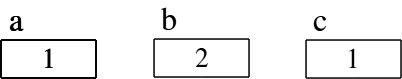
\includegraphics[width=0.8\linewidth,height=0.8\textheight,keepaspectratio=true]{/home/clr/Documents/Cours/DEV1Q2/TDChaine/fr/image/java-logi-egal1.jpg}
						\end{center}
                
                    \caption[java-logi-egal1.jpg]{java-logi-egal1.jpg}
                \end{figure}
                    
            \par
        
        On a : a==c mais a!=b et b!=c
      
            \par
        
			
		\subparagraph{Pour les types r\'ef\'erences} 
		
					\textcolor{white}{.} \par
				
		    Les r\'ef\'erences sont compar\'ees :
		  
            \par
        \begin{figure}[hbt]
				    \begin{center}
					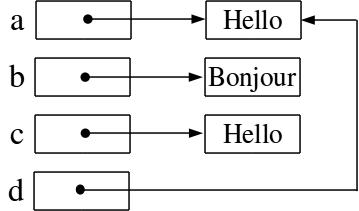
\includegraphics[width=0.8\linewidth,height=0.8\textheight,keepaspectratio=true]{/home/clr/Documents/Cours/DEV1Q2/TDChaine/fr/image/java-logi-egal2.jpg}
						\end{center}
                
                    \caption[java-logi-egal2.jpg]{java-logi-egal2.jpg}
                \end{figure}
                    
            \par
        
        On a : a!=b, a!=c mais a==d
      
            \par
        
			
		\subparagraph{Cas particulier du type String} 
		
					\textcolor{white}{.} \par
				
        Le compilateur r\'eutilise l'espace pour les litt\'eraux de type String
      
            \par
        \begin{Java}
String s1 = "Hello";
String s2 = "Hello";
String s3 = "Hel";
s3 = s3 + "lo";
System.out.println(s1==s2); // Vrai
System.out.println(s1==s3); // Faux
s2 = "Bye";
System.out.println(s1==s2); // Faux
      \end{Java}
			
		\subparagraph{Egalit\'e de valeur : equals()} 
		
					\textcolor{white}{.} \par
				
            \par
        \begin{Java}
String s1 = "Hello";
String s2 = "Hello";
String s3 = "Hel";
s3 = s3 + "lo";
System.out. println (s1. equals(s2 )); // Vrai
System.out. println (s1. equals(s3 )); // Vrai
      \end{Java}
      Ne teste pas que les r\'ef\'erences sont identiques mais bien que les valeurs r\'ef\'erenc\'ees sont \'egales.
      
            \par
        \section{Exercices}
				Maintenant, mettons tout \c ca en pratique.
      
            \par
        \subsection{\`A vous de jouer...}
          N'oubliez pas nos quelques conseils pour vous guider dans la r\'esolution de tels probl\`emes :
          
					\begin{itemize}
				
			\item il convient d'abord de bien comprendre le probl\`eme pos\'e ; assurez-vous qu'il est parfaitement sp\'ecifi\'e ;
			\item r\'esolvez le probl\`eme via quelques exemples pr\'ecis ;
			\item mettez en \'evidence les variables \textbf{\guillemotleft  donn\'ees \guillemotright }, les variables \textbf{\guillemotleft  r\'esultats \guillemotright } et les variables de travail ;
			\item n'h\'esitez pas \`a faire une \'ebauche de r\'esolution en fran\c cais avant d'\'elaborer l'algorithme d\'efinitif pseudo-cod\'e ;
			\item d\'eclarez ensuite les variables (et leur type) qui interviennent dans chaque module ; les noms des variables risquant de ne pas \^etre suffisamment explicites.
			\item \'Ecrivez la partie algorithmique \textbf{AVANT} de vous lancer dans la programmation en Java.
			\item Demandez-vous si vous avez besoin de parcourir tout le tableau ou de sortir pr\'ematur\'ement (si on a trouv\'e ce qu'on cherche par exemple).
			\item Pour la partie Java, dessinez l'arborescence des fichier. 
			\item \textbf{\'Ecrivez le plan de tests en \'ecrivant l'algorithme. Codez les tests apr\`es avoir \'ecrit le code Java.}
					\end{itemize}
				
            \par
        
        \'Ecrivez les algorithmes et codez les programmes Java correspondant qui 
          
					\begin{enumerate}
				
			\item  re\c coit une fraction sous forme de chaine, et retourne la valeur
              num\'erique de celle-ci. Par exemple, si la fraction donn\'ee est "5/8", l'algorithme renverra
              0,625. On peut consid\'erer que la fraction donn\'ee est correcte, elle est compos\'ee de 2 entiers
              s\'epar\'es par le caract\`ere de division '/'.
            
			\item 
              re\c coit le nom complet d'une personne dans une chaine sous la forme
              "nom, pr\'enom" et la renvoie au format "pr\'enom nom" (sans virgule s\'eparatrice). Exemple :
              "De Groote, Jan" deviendra "Jan De Groote".
            
			\item 
              met un mot en \guillemotleft  ou \guillemotright  au pluriel. Pour rappel, un mot en \guillemotleft  ou \guillemotright 
              prend un \guillemotleft  s \guillemotright  \`a l'exception des 7 mots bijou, caillou, chou, genou, hibou, joujou et pou qui
              prennent un \guillemotleft  x \guillemotright  au pluriel. Exemple : un clou, des clous, un hibou, des hiboux. Si le mot
              soumis \`a l'algorithme n'est pas un mot en \guillemotleft  ou \guillemotright , un message ad\'equat sera affich\'e.
              
			\item 
              v\'erifie si un mot donn\'e sous forme de chaine constitue un
              palindrome (comme par exemple "kayak", "radar" ou "saippuakivikauppias" (marchand
              de savon en finnois)
            
			\item 
              v\'erifie si une phrase donn\'ee sous forme de chaine constitue
              un palindrome (comme par exemple "Esope reste ici et se repose" ou "Tu l'as trop
              \'ecras\'e, C\'esar, ce Port-Salut !"). Dans cette seconde version, on fait abstraction des
              majuscules/minuscules et on n\'eglige les espaces et tout signe de ponctuation.
            
			\item 
              re\c coit en param\`etre le tableau avion de n chaines et qui retourne un
              bool\'een indiquant s'il contient au moins un \'el\'ement de valeur \guillemotleft pilote\guillemotright .
            
					\end{enumerate}
				
            \par
        En java, n'oubliez pas d'\'ecrire la javadoc et les tests de vos m\'ethodes.
            \par
        
				\end{document}
			